\documentclass{LS}

% IEEE-style citation and reference formatting
\usepackage{multicol}
\usepackage{graphicx}
\usepackage{caption}
\usepackage{amsmath}
\usepackage{subcaption}
\usepackage{multirow}
\usepackage{booktabs}
\usepackage{float} 
\usepackage{algorithm}
\usepackage{algorithmic}
\usepackage{colortbl}
\usepackage{longtable}
\usepackage{geometry}
\usepackage{array}
\usepackage{tabularx} 
\usepackage{tocloft}
\usepackage{pgfgantt}
\usepackage{hyperref}
\usepackage{soul}
\usepackage{xcolor}
\setulcolor{blue} % Establece el color azul para los subrayados


% IEEE bibliography support
\usepackage{cite}

% Title
\title{\LARGE[PG 251011 ] Desarrollo tecnol\'ogico de un motor rotativo Wankel de 6 tiempos mediante la modelaci\'on termo - mec\'anica de su funcionamiento}

% Authors
\author{
    Juan Jos\'e Rojas Bar\'on\textsuperscript{a,d},
    Vanessa Mar\'ia Serpa P\'aez\textsuperscript{a,d},\\
    Camilo Andres Bayona Roa\textsuperscript{b,d},
}

\begin{document}
\maketitle

\noindent\hrulefill
\vspace{-1em} 
\begin{abstract}

El presente proyecto propone el diseño y modelado termo-mecánico de un motor rotativo tipo Wankel con arquitectura de seis tiempos, como respuesta a la necesidad de mejorar la eficiencia energética y reducir las emisiones contaminantes en motores de combustión interna. Actualmente, los motores Wankel enfrentan limitaciones como el bajo aprovechamiento térmico y la alta emisión de hidrocarburos no quemados (uHC), consecuencia directa de su geometría interna. A pesar de su alta densidad de potencia y compacidad, su adopción ha sido restringida por estos factores. La relevancia de abordar esta problemática radica en el potencial de reaprovechar la energía térmica y los uHC mediante una segunda combustión controlada, lo cual permitiría reducir el consumo específico de combustible y mejorar el rendimiento global sin añadir más combustible al sistema. Para ello, se desarrollará una herramienta computacional \textcolor{blue}{por medio de lenguajes de programación} que permita simular el comportamiento del motor \textcolor{blue}{bajo parámetros geométricos que puedan modificarse para analizar o diseñar estas tecnologías.} Esta herramienta integrará modelos matemáticos de presión, temperatura y volumen \textcolor{blue}{y cinética de combustión} a lo largo del ciclo completo, incluyendo las fases adicionales propuestas. Se espera que el motor Wankel de seis tiempos, al incorporar una segunda fase de admisión, compresión y combustión, logre un incremento significativo en la eficiencia térmica y una disminución de las emisiones contaminantes, abriendo nuevas posibilidades para su implementación en aplicaciones donde el espacio, el peso y la autonomía energética son críticos.

\end{abstract}
\vspace{-1em} 

\begin{center}
\textbf{\textit{\fontsize{8}{10}\selectfont Keywords:}} \textit{\fontsize{8}{10}\selectfont   Motor Wankel, seis tiempos, combustión secundaria, hidrocarburos no quemados (uHC), eficiencia térmica, simulación computacional, modelado termo-mecánico. }
\end{center}

\noindent\hrulefill

% Main Content

\section{\bfseries\fontsize{10}{12}\selectfont Justificación y planteamiento del problema  }\label{sec:intro}

La humanidad enfrenta actualmente el reto de transformar y utilizar la energía de forma más eficiente y sostenible. La demanda energética mundial ha aumentado de manera sostenida debido al crecimiento poblacional, la digitalización y la electrificación de procesos, alcanzando un incremento del 2.2\% solo en 2024, impulsado principalmente por el sector eléctrico, que creció un 4.3\% de acuerdo con \cite{iea2025a,iea2025b}. Este consumo intensivo, todavía dominado por los combustibles fósiles, es responsable de aproximadamente el 42\% de las emisiones globales de gases de efecto invernadero según \cite{ipcc2022a,ipcc2022b}. Frente a este panorama, la transición energética se ha convertido en un imperativo técnico y ético, impulsando el desarrollo de nuevas tecnologías que logren una conversión energética más eficiente como lo mencionan \cite{perino2021}.

Entre las tecnologías de conversión energética, los motores de combustión interna siguen teniendo una participación considerable a nivel global. En 2023, los combustibles fósiles representaron aproximadamente el 80\% de la demanda energética mundial, lo que refleja el papel predominante que aún juegan los motores térmicos en el transporte y la industria de acuerdo con \cite{iea2024}. En este contexto, el motor rotativo Wankel destaca por su alta densidad de potencia, diseño compacto, menor número de partes móviles y operación suave. Según \cite{cole1972}, el motor Wankel presenta la ventaja de realizar de forma simultánea tres fases diferentes del ciclo termodinámico: admisión, compresión y expansión, en sus respectivas cámaras, lo que contribuye a una entrega de potencia más fluida y constante, además de operar con menos fricción y menor peso. En la figura 1 se describen los componentes principales del motor Wankel de cuatro tiempos, así como su funcionamiento.

\begin{figure}[H]
    \centering
    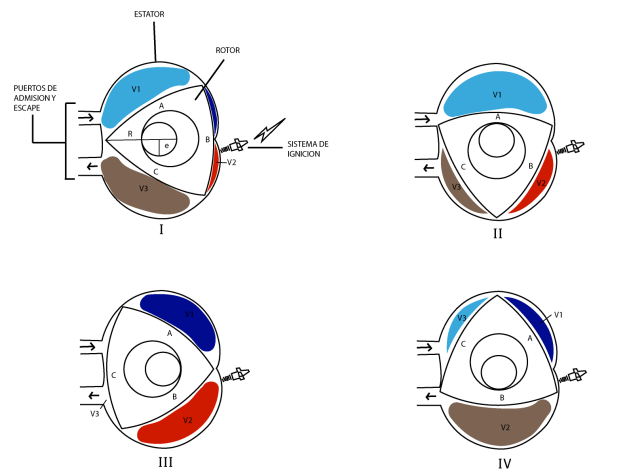
\includegraphics[width=0.55\textwidth]{imagenes/Wankel.png}
    \caption{Ciclo básico de funcionamiento del motor Wankel de cuatro tiempos. Tomado de \cite{canals2011}, p. 9.}
    \label{fig:geometria-yamamoto}
\end{figure}

Sin embargo, una de las particularidades más críticas del diseño del motor Wankel es la necesidad de inyectar aceite directamente en la cámara de combustión para lubricar los sellos del rotor, lo cual genera un consumo de aceite significativamente más alto en comparación con los motores de pistones \cite{elbahja2023}. Esta característica de diseño, junto con otros desafíos técnicos, ha limitado históricamente su aplicación. Entre estos se destacan su baja eficiencia térmica, las elevadas emisiones de hidrocarburos no quemados (uHC) y el ya mencionado consumo elevado de aceite.

En un estudio comparativo entre un motor rotativo Mazda 13B de 1308 cm\textsuperscript{3} y un motor de pistones Buick V6 de 3777 cm\textsuperscript{3}, ambos con potencias similares, \cite{cole1976} encontraron que el motor Wankel presentaba emisiones de hidrocarburos entre 6 y 10 veces superiores. Estas deficiencias fueron atribuidas a la geometría alargada de la cámara de combustión, particularmente por su alta relación superficie-volumen y la dificultad de acceso de la llama a ciertas zonas de la mezcla, lo que favorece una combustión incompleta y, por consiguiente, un aumento significativo en la generación de hidrocarburos no quemados de acuerdo con \cite{yamamoto1972}. 

De acuerdo con \cite{kuppa2019}, en motores de pistones los uHC generados por crevices pueden alcanzar concentraciones de hasta 1100 ppm, y los causados por el apagamiento de llama en la pared hasta 600 ppm, dando un total aproximado de 1700 ppm. Considerando la proporción reportada por \cite{cole1976}, según la cual los motores Wankel emiten entre 6 y 10 veces más uHC, se puede estimar que estos podrían alcanzar concentraciones entre 10200 ppm y 17 000 ppm.


Complementariamente, un estudio realizado por la NASA comparó motores Wankel con motores de pistones de aviación bajo condiciones operativas equivalentes, y halló que el consumo específico de combustible al freno (BSFC) del motor rotativo fue entre un 15\% y 20\% más alto. Esta diferencia refleja una conversión menos eficiente de la energía del combustible en trabajo útil \cite{nasa1984}.


A partir de esta problemática, emerge una oportunidad de innovación: aprovechar energéticamente los uHC y el calor residual de la primera etapa mediante una segunda combustión controlada, lo que permitiría incrementar la eficiencia global del sistema, reducir el impacto ambiental y generar trabajo adicional sin necesidad de inyectar más combustible. Para ello, surgen propuestas de rediseño del ciclo termodinámico convencional de cuatro tiempos, como el motor Wankel de seis tiempos, que incorpora etapas adicionales de admisión y expansión. Su desarrollo requiere herramientas de simulación adaptadas a un comportamiento no convencional, tanto en la dinámica de volúmenes como en el tratamiento de la combustión residual. Esta idea se fundamenta en el análisis geométrico realizado por Yamamoto en su obra \textit{Rotary Engine}, donde se documentan variaciones sobre la curva epitrocoidal que constituye la base del motor Wankel de cuatro tiempos, incluyendo la factibilidad de incorporar tiempos adicionales, en la Figura 2 se observa la geometría del motor Wankel de cuatro tiempos (2) y la geometría que cumple con las condiciones para llevar a cabo los seis tiempos (3).

\begin{figure}[H]
    \centering
    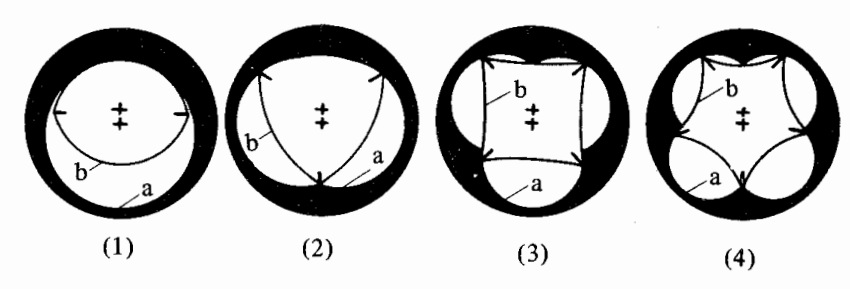
\includegraphics[width=0.5\textwidth]{imagenes/4 y 6.png}
    \caption{Comparación de variaciones geométricas en el diseño del motor Wankel. Tomado de \textcite{yamamoto1971}, p. 9.}
    \label{fig:geometria-yamamoto}
\end{figure}

Actualmente, no existen motores rotativos Wankel de seis tiempos con una segunda fase de combustión para el aprovechamiento de los uHC desarrollados ni documentados en la literatura, lo que convierte esta configuración en una propuesta completamente original. A su vez, tampoco se dispone de herramientas computacionales ni modelos termodinámicos generalizados que permitan analizar, simular u optimizar el comportamiento de este tipo de arquitectura extendida, lo cual representa una barrera técnica significativa y una brecha relevante en la investigación actual.

\textcolor{blue}{La ejecución de este proyecto tiene implicaciones significativas tanto en el ámbito teórico como en aplicaciones reales. Desde la perspectiva académica, el desarrollo de una herramienta computacional para modelar un motor Wankel de seis tiempos representa un aporte inédito, al proponer un marco de simulación adaptable a configuraciones rotativas no convencionales. Esta herramienta permitirá analizar fenómenos asociados a la termodinámica de doble combustión, evaluar diferentes geometrías y optimizar el desempeño del ciclo, abriendo nuevas líneas de investigación en el campo de las máquinas térmicas. En el plano práctico, el diseño propuesto puede aplicarse en escenarios donde el espacio, el peso y la eficiencia energética son factores críticos, como en sistemas de movilidad eléctrica, generadores compactos o vehículos aéreos no tripulados. En la actualidad, los motores Wankel se emplean en diversas tecnologías gracias a su compacidad, bajo peso y elevada densidad de potencia. Un ejemplo es el Mazda MX-30 e-Skyactiv R-EV, que incorpora un motor rotativo como generador para recargar baterías, combinando la eficiencia de la propulsión eléctrica con la versatilidad térmica \cite{mazda2023}. En el ámbito militar, la empresa AIE ha desarrollado el motor rotativo 225CS para UAVs, con capacidad multifuel y alta relación potencia-peso \cite{aie2024}. Por su parte, la compañía LiquidPiston diseñó el motor X Mini, de 70 cc, destacando por su eficiencia energética, compacidad y capacidad para operar con distintos combustibles, siendo ideal para generadores portátiles y vehículos ligeros \cite{liquidpiston2024}.
}.


En este contexto, el desarrollo de un motor Wankel de seis tiempos otorgaría mejoras que serían especialmente valiosas en las aplicaciones mencionadas, donde el espacio y la autonomía energética son críticos, posicionando a esta arquitectura como una alternativa prometedora para la siguiente generación de tecnologías compactas, híbridas o portátiles. Así, el proyecto no solo busca resolver una necesidad técnica no atendida, sino también abrir el camino hacia soluciones energéticas más  eficientes y adaptables a contextos tecnológicos emergentes.



\section{\bfseries\fontsize{10}{12}\selectfont Antecedentes} \label{sec:intro} 

\textcolor{blue}{Desde tiempos antiguos, la humanidad ha buscado transformar la energía natural de manera más eficiente, comenzando con la fuerza humana y animal, y luego aprovechando fuentes como el viento y el agua mediante dispositivos como molinos y norias \cite{pacheco2015, kandari2013}. La invención de la máquina de vapor en el siglo XVIII permitió convertir calor en trabajo mecánico continuo, impulsando la Revolución Industrial y el uso intensivo de combustibles fósiles \cite{pacheco2015}. Posteriormente, en el siglo XIX, surgieron los motores de combustión interna, que transforman la energía química de los combustibles en movimiento rotativo, sentando las bases de la ingeniería energética moderna \cite{morocho2023}. Estos motores se han consolidado en transporte, industria y generación eléctrica, con mejoras continuas en eficiencia y emisiones. Los motores Otto y Diesel alcanzan eficiencias ideales de 25–30\% y hasta 45\%, respectivamente \cite{guzzella2010, olivier2021}}.


Desde su invención, los motores de combustión interna han evolucionado principalmente en configuraciones de dos y cuatro tiempos, ampliamente utilizadas en aplicaciones móviles e industriales. El motor de dos tiempos completa un ciclo de admisión, compresión, combustión y escape en una sola vuelta del cigüeñal, lo que le permite generar más potencia por unidad de volumen. Específicamente, estos motores pueden producir aproximadamente un 17\,\% más de potencia en comparación con motores de cuatro tiempos de tamaño similar acorde con lo que menciona \cite{amet2002}. Sin embargo, esta mayor potencia conlleva desventajas significativas: los motores de dos tiempos suelen consumir más combustible y emitir mayores niveles de contaminantes. De hecho, se ha observado que las emisiones de hidrocarburos en motores de dos tiempos pueden ser hasta seis veces superiores a las de motores de cuatro tiempos  según \cite{downtoearth2001}.

\begin{figure}[H]
    \centering
    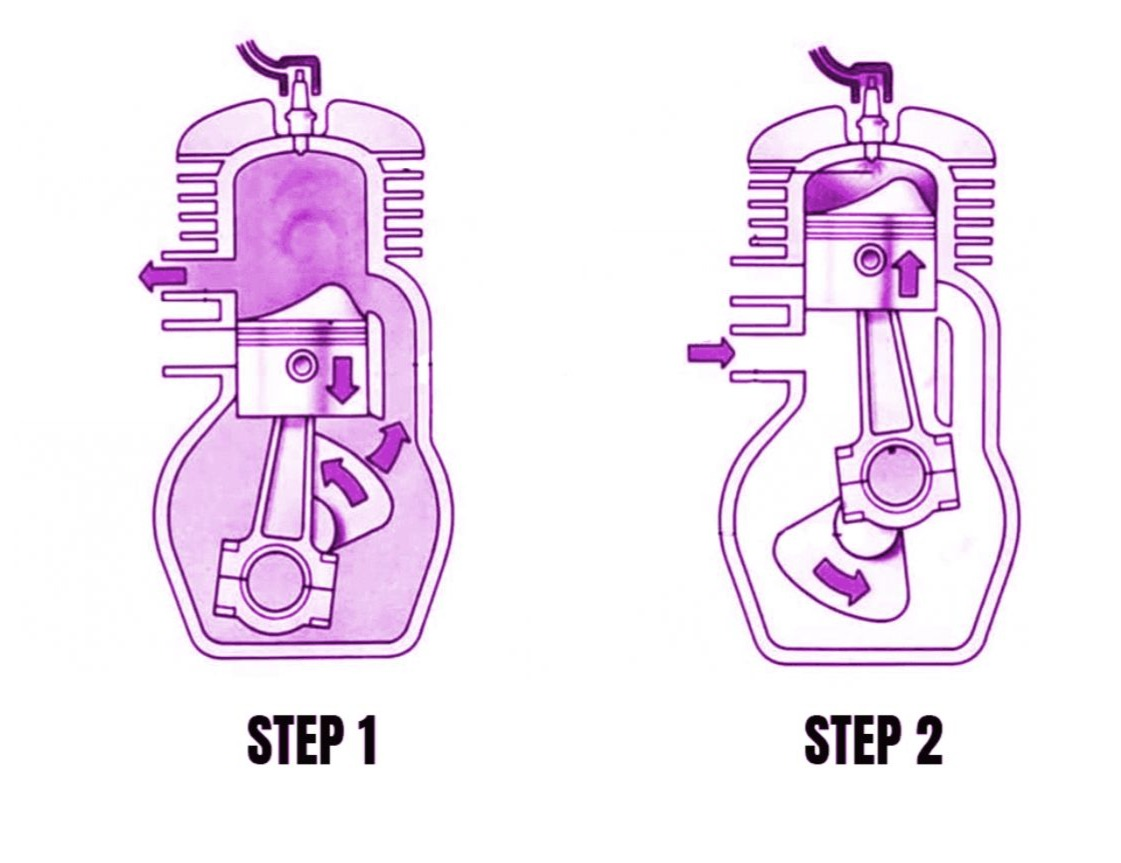
\includegraphics[width=0.3\textwidth]{imagenes/2tiempos.jpg}
    \caption{Ciclo básico de funcionamiento del motor de dos tiempos. Tomado de \cite{jcosta2t}}
    \label{fig:2tiempos}
\end{figure}

Por otro lado, el motor de cuatro tiempos distribuye las fases de admisión, compresión, combustión y escape en dos vueltas completas del cigüeñal. Esta configuración mejora la eficiencia térmica y reduce las emisiones contaminantes. Estudios indican que los motores de cuatro tiempos pueden ser hasta un 50\,\% más eficientes en el consumo de combustible que sus contrapartes de dos tiempos de acuerdo con \cite{boatersworld2023}. Además, las emisiones de hidrocarburos en motores de cuatro tiempos son significativamente menores, representando solo una fracción de las emitidas por motores de dos tiempos de acuerdo con \cite{downtoearth2001}.

\begin{figure}[H]
    \centering
    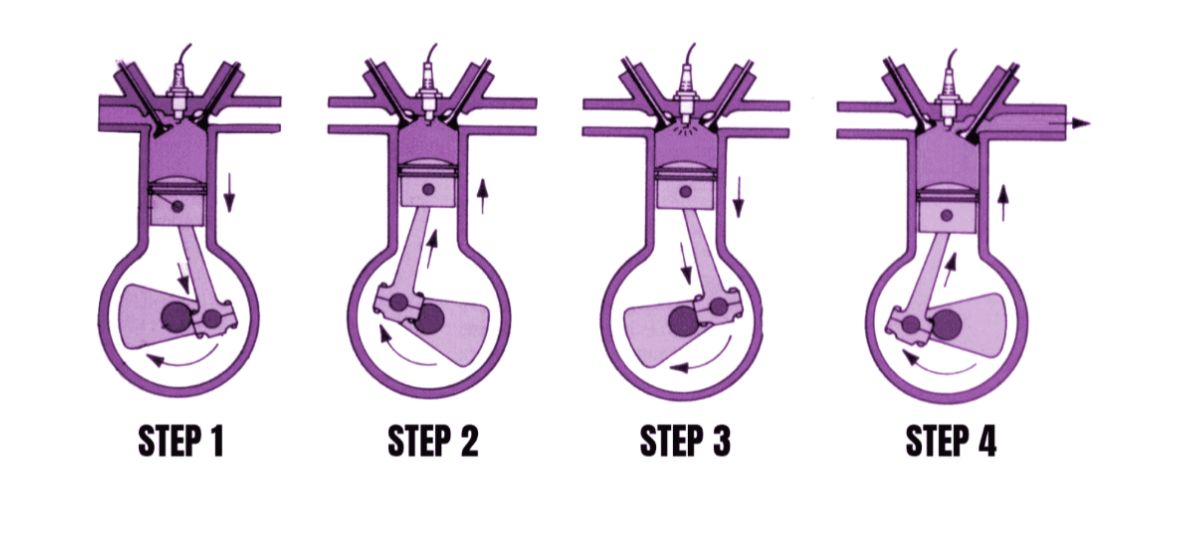
\includegraphics[width=0.5\textwidth]{imagenes/4tiempos.jpg}
    \caption{Ciclo básico de funcionamiento del motor de cuatro tiempos. Tomado de \cite{jcosta4t}}
    \label{fig:4tiempos}
\end{figure}

Ambos tipos de motores presentan una sola combustión por ciclo y una única expansión del gas, lo que limita el aprovechamiento energético total como lo menciona \cite{fiveable2023}. Estas limitaciones justifican la aparición de configuraciones extendidas como los motores de seis tiempos, que permiten incorporar etapas adicionales para recuperar calor o limpiar la cámara de combustión, aumentando así la eficiencia global del ciclo de acuerdo con \cite{kandari2013, bajulaz1989}.

El motor de seis tiempos desarrollado por Roger Bajulaz en 1989 introduce dos etapas adicionales al ciclo convencional de cuatro tiempos: una segunda expansión y un segundo escape. Tras la fase de escape tradicional, se inyecta agua fría en la cámara de combustión caliente. Esta agua se vaporiza instantáneamente debido al calor residual, generando una expansión adicional que produce trabajo útil sin consumo extra de combustible. Este proceso no solo mejora la eficiencia térmica del motor, sino que también contribuye a la reducción de la temperatura de operación y de las emisiones contaminantes. Estudios indican que la inyección de agua en motores de seis tiempos puede reducir la temperatura de la culata hasta en un 50\%, lo que disminuye la necesidad de sistemas de enfriamiento convencionales. Además, se ha observado una disminución en el consumo de combustible de al menos un 40\% y una reducción significativa en las emisiones de óxidos de nitrógeno (NOx) y otros contaminantes como se menciona en \cite{review2017}.

\begin{figure}[H]
    \centering
    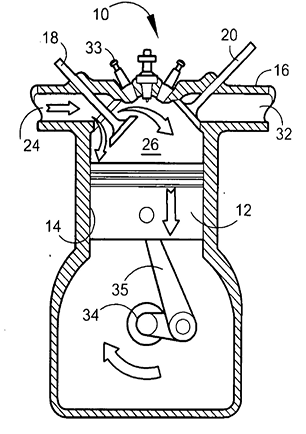
\includegraphics[width=0.2\textwidth]{imagenes/bajulaz.png}
    \caption{Motor Bajulaz de seis tiempos. Tomado de \cite{bajulaz1989}}
    \label{fig:bajulaz}
\end{figure}

El motor Velozeta, por su parte, añade dos fases adicionales orientadas a limpieza y enfriamiento del cilindro. Tras la combustión y escape tradicionales, el motor introduce una fase de barrido con aire comprimido, y luego una fase de refrigeración, también con aire, antes de repetir el ciclo. Estas etapas estabilizan térmicamente el sistema, aunque no generan trabajo adicional como en el caso de Bajulaz de acuerdo con \cite{pande2015}.

\begin{figure}[H]
    \centering
    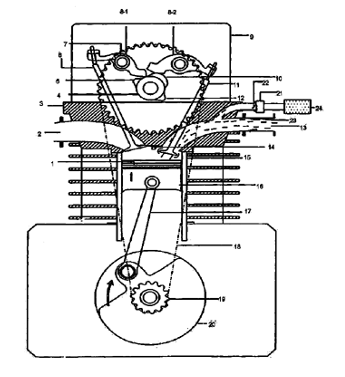
\includegraphics[width=0.23\textwidth]{imagenes/velozeta.png}
    \caption{Motor Velozeta de seis tiempos. Tomado de \cite{pande2015}}
    \label{fig:velozeta}
\end{figure}

En 2024, Porsche patentó un motor de seis tiempos que introduce un sistema de excentricidad en el cigüeñal, permitiendo al pistón alcanzar dos puntos muertos inferiores distintos durante el ciclo. Esta geometría habilita una segunda compresión tras la fase de escape, mediante la admisión de aire fresco a través de puertos laterales, justo cuando el pistón llega al punto más bajo. Esta segunda mezcla se combina con los hidrocarburos no quemados (uHC) de la combustión anterior, permitiendo una nueva ignición sin inyección adicional de combustible según \cite{porsche2024}.

\begin{figure}[H]
    \centering
    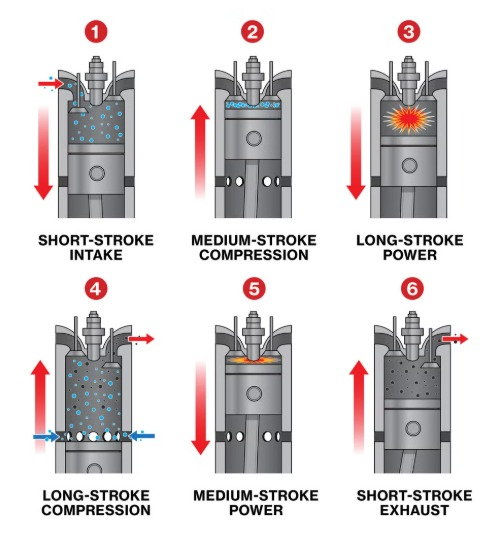
\includegraphics[width=0.35\textwidth]{imagenes/porshe.jpg}
    \caption{Motor Porsche de seis tiempos. Tomado de \cite{porsche2024}}
    \label{fig:porsche}
\end{figure}

El motor X desarrollado por LiquidPiston implementa el ciclo híbrido de alta eficiencia (HEHC), combinando elementos de los ciclos Otto, Diesel y Atkinson. Este motor rotativo presenta un rotor con forma de lóbulos que gira dentro de una carcasa triangular fija, realizando los procesos de admisión, compresión, combustión y escape en tres cámaras separadas. Una característica destacada del motor X es su capacidad para operar con una relación de compresión elevada. En los prototipos de encendido por compresión (CI-HEHC), se han alcanzado relaciones de compresión de hasta 26:1, lo que mejora significativamente la eficiencia térmica del motor de acuerdo con \cite{liquidpiston2023}. Además, el diseño del motor permite una combustión cercana a condiciones de volumen constante. Esto se logra mediante una detención cerca del punto muerto superior, que prolonga el tiempo disponible para la combustión. Esta característica, junto con la alta relación de compresión, contribuye a una mejor gestión térmica y a una reducción en el tiempo de combustión, optimizando el rendimiento del motor de acuerdo con \cite{liquidpiston2023}.

\begin{figure}[H]
    \centering
    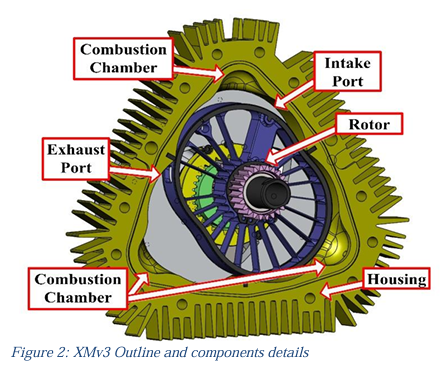
\includegraphics[width=0.3\textwidth]{imagenes/liquid.png}
    \caption{Motor LiquidPiston XMv3. Tomado de \cite{liquidpiston2015}}
    \label{fig:liquidpiston}
\end{figure}

El segundo caso son los motores \textit{rotary vane} o de paletas rotativas. En estos diseños, un rotor central gira dentro de una carcasa con forma excéntrica y posee varias paletas móviles que se expanden radialmente hacia las paredes internas de la carcasa. Estas paletas dividen el espacio en múltiples cámaras de trabajo que varían de volumen a medida que el rotor gira, permitiendo realizar de forma continua las etapas del ciclo: admisión, compresión, combustión y escape. Su diseño compacto, con pocas piezas móviles—generalmente cuatro: el rotor, la carcasa y dos paletas deslizantes como lo menciona \cite{csef2012} y rotación continua, proporciona una entrega de energía estable y un potencial de alto rendimiento volumétrico. Sin embargo, enfrentan desafíos de sellado dinámico, especialmente en las paletas, así como problemas de desgaste y eficiencia térmica a altas cargas como lo menciona \cite{sharma2017}. Recientemente, se ha patentado un diseño de motor rotary vane de seis tiempos, el cual añade dos etapas adicionales de expansión y escape. El sistema cuenta con cámaras distribuidas alrededor del rotor que permiten gestionar por separado la primera y segunda combustión, así como los gases residuales. Las válvulas de control y las geometrías internas están diseñadas para secuenciar los seis tiempos sin interrupción del giro de acuerdo con \cite{vane6t2022}.

\begin{figure}[H]
    \centering
    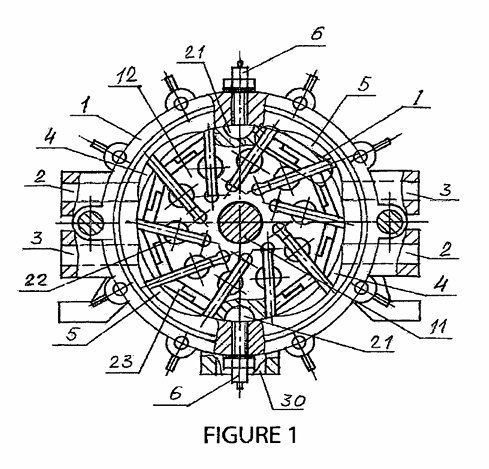
\includegraphics[width=0.4\textwidth]{imagenes/vane6.png}
    \caption{Motor Rotary Vane de seis tiempos. Tomado de \cite{vane6t2022}}
    \label{fig:vane}
\end{figure}

A diferencia de estos desarrollos, la presente propuesta plantea un motor rotativo tipo Wankel con seis tiempos, que conserva la arquitectura rotativa original pero añade una segunda fase de admisión, compresión y combustión. Esto permitiría reaprovechar los hidrocarburos no quemados (uHC) de la primera combustión, generando una nueva ignición sin añadir combustible adicional, lo cual no ha sido documentado ni implementado en configuraciones rotativas actuales. Así, este proyecto aborda una brecha tecnológica real en el desarrollo de motores rotativos de múltiples tiempos, al tiempo que propone una nueva herramienta de modelado computacional adaptada a esta arquitectura no convencional.


\section{\bfseries\fontsize{10}{12}\selectfont Objetivos }\label{sec:intro}

\textit{Desarrollar una herramienta computacional que permita modelar el comportamiento termomecánico de un motor rotativo tipo Wankel de seis tiempos, mediante la formulación de modelos analíticos y numéricos, así como su codificación en lenguajes de programación como Python para apoyar tareas de diseño mediante la variación de parámetros geométricos.}


\begin{enumerate}
    \setlength{\itemsep}{0pt}
    \setlength{\parskip}{0pt}
    
    \item Concebir las definiciones mecánicas del ciclo de seis tiempos en un motor Wankel, identificando sus fases operativas y las variables clave para su modelado numérico.

    \item Formular un modelo matemático que represente el comportamiento termo-mecánico del motor Wankel, considerando los procesos de admisión, compresión, combustión, expansión, postcompresión, postcombustión y postexpansión.

    \item Implementar el modelo matemático mediante una herramienta computacional desarrollada en Python y/o MATLAB, estructurada de forma modular y orientada a la simulación del ciclo termodinámico completo.

    \item Operar la herramienta computacional desarrollada para analizar el desempeño de multiples diseños del motor Wankel de seis tiempos operando en distintos escenarios, evaluando geometrías del rotor y estator.

    %\item Ejecutar simulaciones con la herramienta computacional desarrollada para analizar el desempeño de diferentes configuraciones del motor Wankel de seis tiempos, evaluando parámetros geométricos del estator y del rotor, %así como variables de operación como presión, temperatura, volumen, eficiencia térmica y trabajo útil generado.
    
\end{enumerate}

\subsection{Declaración de diseño}

Se propone el diseño de una herramienta computacional que permita modelar y analizar el comportamiento termomecánico de un motor rotativo tipo Wankel con arquitectura de seis tiempos. Esta herramienta estará orientada a la simulación de los procesos de admisión, compresión, combustión, expansión y postcompresión, postcombustión, postexpansión, incorporando la reutilización de hidrocarburos no quemados (uHC) como estrategia para mejorar la eficiencia térmica y reducir las emisiones contaminantes.

El diseño integra el desarrollo de modelos matemáticos y termodinámicos del ciclo de seis tiempos, programados en entornos como Python y MATLAB, con el fin de facilitar su implementación, validación y análisis bajo diferentes condiciones de operación. La herramienta incluirá un entorno de simulación modular que permitirá visualizar parámetros como presión, volumen, temperatura, trabajo y eficiencia, en función de variables controlables.

Esta propuesta no busca replicar un motor existente, sino explorar una arquitectura que hasta la fecha no ha sido documentada: un motor rotativo tipo Wankel con seis tiempos. El diseño se justifica por su potencial de innovación técnica, energética y ambiental, y se considera una contribución al desarrollo de herramientas de simulación adaptadas a ciclos termodinámicos extendidos.


\subsection{Requerimientos esperados de diseño}

La herramienta computacional propuesta deberá cumplir con los siguientes requerimientos técnicos para ser considerada funcional y validada como un diseño de ingeniería:

\begin{enumerate}
    \item \textbf{Simulación completa del ciclo termomecánico}: Reproducir de forma lógica y coherente las seis fases del motor propuesto (incluyendo la segunda combustión), con continuidad temporal y conservación de la energía.
    
    \item \textbf{Cálculo de variables clave}: Calcular la cinemática del sistema Rotor - Estator así como presión, volumen, temperatura, trabajo y eficiencia térmica durante cada fase, con exactitud teórica y consistencia entre ciclos.
    
    \item \textbf{Capacidad de análisis paramétrico}: Permitir la modificación de parámetros de entrada como la geometría variando la relación de compresión, así como temperatura inicial, tipo de mezcla, presencia de uHC y tiempos de apertura simulados.
    
    \item \textbf{Representación gráfica del comportamiento del sistema}: Generar al menos dos tipos de gráficas para interpretar el comportamiento del ciclo: curvas presión-volumen (P--V) y evolución térmica (T vs. tiempo o T--s).
    
    \item \textbf{Confiabilidad numérica}: El modelo debe presentar estabilidad numérica y resultados reproducibles ante variaciones controladas en las condiciones iniciales.
    
    \item \textbf{Entrega de datos interpretables}: Exportar o mostrar resultados en formato numérico organizado (tablas o listas) que puedan ser analizados técnica o comparativamente.
    
    \item \textbf{Ejecutabilidad autónoma}: Ser un código que funcione sin intervención constante, cargue los parámetros de entrada desde archivos o scripts y devuelva resultados claros al usuario.
\end{enumerate}

\vspace{1em}
\subsection{Restricciones de diseño (Factibilidad)}

El desarrollo de la herramienta computacional propuesta enfrenta varias restricciones que limitan su alcance, complejidad y nivel de validación durante el proyecto de grado:

\begin{itemize}
    \item \textbf{Limitaciones computacionales}: El desarrollo y validación del modelo está limitado a los recursos de procesamiento disponibles en equipos personales, lo cual puede restringir la resolución numérica o la capacidad de visualización avanzada de resultados.
    
    \item \textbf{Falta de datos experimentales específicos}: Al tratarse de una arquitectura rotativa no documentada previamente, no se cuenta con información empírica directa para comparación, lo que obliga a validar el modelo mediante estimaciones teóricas y supuestos razonables.
    
    \item \textbf{Tiempo académico limitado}: El trabajo de grado debe realizarse dentro del calendario académico establecido, lo que condiciona el nivel de detalle y profundidad que puede alcanzar el diseño y su implementación.
    
    \item \textbf{Restricciones de acceso a software licenciado}: Aunque herramientas como MATLAB ofrecen entornos potentes para simulación, se priorizará el uso de lenguajes libres como Python para asegurar la accesibilidad y continuidad del proyecto sin depender de licencias institucionales.
\end{itemize}

\subsection{Normas y estándares (Buenas prácticas)}

El diseño propuesto se alineará con estándares y buenas prácticas aplicables al desarrollo de simulaciones termodinámicas de motores rotativos, considerando los siguientes referentes:

\begin{itemize}
    \item \textbf{ISO 15550:2002} – \cite{iso15550} establece los lineamientos para la determinación de la potencia efectiva en motores de combustión interna alternativos. Aunque se orienta principalmente a motores con pistones, sus principios son útiles como referencia para evaluar el desempeño térmico y mecánico en simulaciones de ciclos complejos como el de seis tiempos.

    \item \textbf{SAE J1349} – De acuerdo con \cite{saeJ1349}, este estándar define las condiciones para la medición de la potencia neta en motores de encendido por chispa y compresión. Su aplicación en simulaciones permite verificar la coherencia y realismo de los resultados obtenidos bajo parámetros estandarizados.

    \item \textbf{ISO/IEC 25010:2011} – Esta norma establece un modelo de calidad para productos de software, incluyendo atributos como funcionalidad, fiabilidad, usabilidad, eficiencia de desempeño, mantenibilidad y portabilidad. Su adopción en el presente proyecto asegura que el desarrollo de la herramienta computacional siga buenas prácticas en codificación, validación y documentación \cite{iso25010}.

\end{itemize}

\section{\bfseries\fontsize{10}{12}\selectfont Caso de estudio  }\label{sec:intro}

El caso de estudio se basa en la simulación de un motor rotativo tipo Wankel de seis tiempos, cuya arquitectura será diseñada y modelada computacionalmente como parte de este proyecto. Para evaluar su desempeño, se realizará una comparación directa con un motor Wankel de cuatro tiempos previamente simulado en el marco de la asignatura de Máquinas Térmicas presentado en el Anexo 1, bajo condiciones iniciales equivalentes y parámetros geométricos similares. El análisis se centrará en variables como eficiencia térmica, trabajo útil generado y aprovechamiento energético. Dado que el diseño de seis tiempos no ha sido documentado, su validación se realizará mediante escenarios virtuales.



\section{\bfseries\fontsize{10}{12}\selectfont Metodología }\label{sec:metodologia}

Para cumplir con los objetivos propuestos, se desarrollarán una serie de actividades estructuradas en función del ciclo de diseño, implementación y validación de la herramienta computacional.

En primera instancia, se realizará el diseño geométrico del motor rotativo tipo Wankel de seis tiempos. Esta etapa contempla la definición de la carcasa, el perfil del rotor, y la relación geométrica entre ambos, considerando parámetros como el radio del círculo base, la excentricidad y la relación de compresión. A partir de estas dimensiones, se derivarán las ecuaciones que describen el cambio de volumen dentro de la cámara de combustión durante el movimiento relativo del rotor. Estas ecuaciones permitirán construir el ciclo presión-volumen (P–V) característico del motor propuesto.

Posteriormente, se formulará un modelo matemático y termodinámico que represente las seis fases del motor, incluyendo una segunda admisión, compresión,combustión y expansión. El modelo será construido utilizando balances de masa y ecuaciones de estado, respetando principios de conservación de masa y energía. Dado que no existen modelos previos para esta arquitectura, los métodos serán adaptados a partir de referencias de motores convencionales, integrando supuestos razonables y condiciones límite de operación.

Una vez estructurado el modelo teórico, se procederá con la implementación computacional de la herramienta en lenguajes como Python y MATLAB. Esta herramienta será construida de forma modular, permitiendo la simulación de cada fase del ciclo y la configuración flexible de parámetros como la geometría del motor, la presencia de hidrocarburos no quemados (uHC), y condiciones iniciales de temperatura y presión. Se garantizará la trazabilidad del código y su validación interna mediante pruebas de consistencia numérica.

A continuación, se ejecutarán simulaciones en distintos escenarios definidos por variaciones en parámetros geométricos y termodinámicos del sistema. Los parámetros geométricos incluirán el radio del círculo base del rotor, la excentricidad, la altura del rotor, el espesor de la carcasa y la relación volumen mínimo-volumen máximo por cámara. Por su parte, los parámetros termodinámicos considerados serán la temperatura y presión inicial en la segunda admisión, la composición de la mezcla aire-combustible, la presencia de hidrocarburos no quemados (uHC) y el calor específico de los gases involucrados. Estas simulaciones permitirán analizar la evolución temporal del ciclo de seis tiempos y su efecto en el desempeño del motor. Los resultados se organizarán en gráficos presión-volumen (P--V), temperatura versus angulo (T--$\theta$), presion versus angulo (P--$\theta$), acompañados de tablas numéricas que facilitarán su interpretación técnica.

Finalmente, se evaluará si la herramienta desarrollada reproduce de manera coherente el comportamiento termodinámico esperado del motor, y si permite comparar distintos diseños o configuraciones con base en criterios de eficiencia térmica, trabajo útil generado y comportamiento volumétrico. Los hallazgos serán documentados siguiendo principios de trazabilidad, mantenibilidad y calidad del software, en concordancia con la norma ISO/IEC 25010:2011.



\begin{table}[H]
    \centering
    \tiny % Reduce aún más el tamaño de la fuente
    \renewcommand{\arraystretch}{0.8} % Ajusta la separación vertical de las filas

    \begin{tabular}{p{2.6cm} p{3.5cm} p{3.5cm} p{3cm}}
        \hline
        \textbf{Objetivo} & \textbf{Actividades} & \textbf{Herramientas de Ingeniería} & \textbf{Entregable} \\
        \hline

        Definir las características mecánicas y termodinámicas del ciclo de seis tiempos en un motor Wankel &
        - Diseñar geométricamente la carcasa y el rotor \newline
        - Formular ecuaciones que describan el cambio de volumen en función del ángulo &
        - Referencias técnicas (Yamamoto) \newline
        - Herramientas de dibujo técnico \newline
        - Principios de diseño de motores rotativos &
        - Modelo geométrico base \newline
        - Ecuaciones funcionales del volumen \\

        \hline

        Formular un modelo matemático del comportamiento termomecánico del motor &
        - Establecer balances de masa y energía \newline
        - Incluir procesos de admisión, compresión, combustión y postcombustión &
        - Leyes de la termodinámica \newline
        - Ecuaciones de estado \newline
        - Modelado físico-matemático &
        - Sistema de ecuaciones del ciclo \newline
        - Definición de fases operativas \\

        \hline

        Implementar el modelo computacionalmente &
        - Codificar en Python/MATLAB \newline
        - Integrar parámetros modificables \newline
        - Validar funcionamiento numérico &
        - Programación modular \newline
        - Simulación dinámica \newline
        - Pruebas de consistencia &
        - Código ejecutable funcional \newline
        - Documentación del modelo \\

        \hline

        Ejecutar simulaciones y analizar el desempeño del diseño &
        - Simular distintos escenarios geométricos y termodinámicos \newline
        - Generar gráficas P--V, T--$\theta$ y P--$\theta$\newline
        - Evaluar eficiencia térmica y trabajo útil &
        - Simulación computacional \newline
        - Visualización gráfica \newline
        - Estadística básica &
        - Informe técnico de análisis \newline
        - Resultados numéricos y gráficos \\

        \hline
    \end{tabular}
    \caption{\textit{Resumen de actividades por objetivo específico. Elaboración propia.}}
    \label{tab:resumen_actividades}
\end{table}



\section{\bfseries\fontsize{10}{12}\selectfont Cronograma} 

\label{sec:intro} \begin{figure}[H]
    \centering
    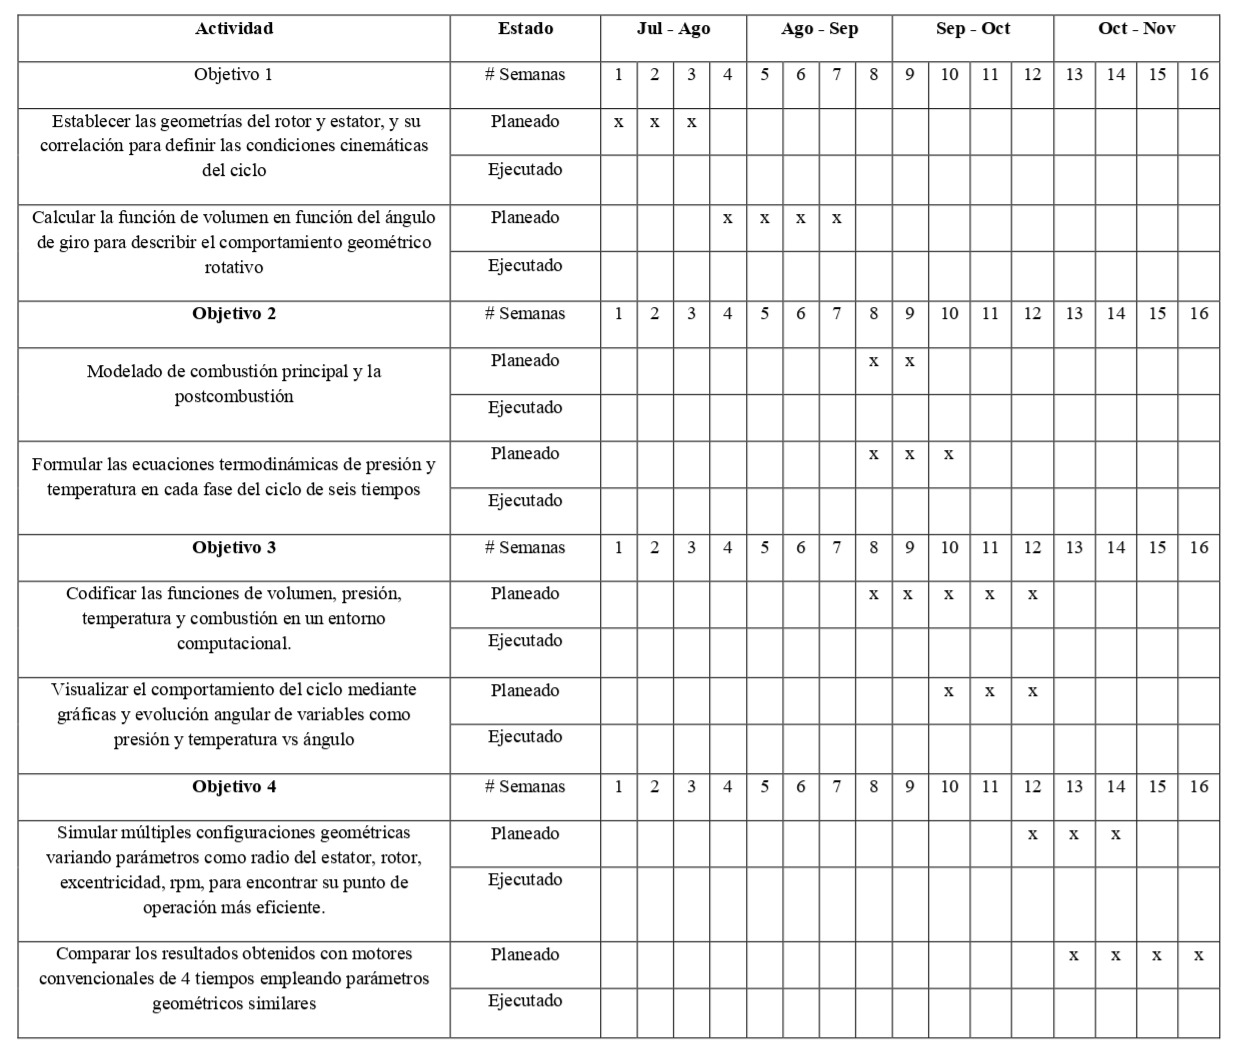
\includegraphics[width=1\textwidth]{imagenes/Gantt_page-0001.jpg}
    \textbf{Tabla 2}. \textit{Diagrama de Gantt}
    \label{fig:liquidpiston}
\end{figure}

\vspace{1em}
\noindent\textbf{Nota:} Las celdas marcadas con \textbf{x} indican las semanas en que se prev\'e el desarrollo de cada actividad.

\section{\bfseries\fontsize{10}{12}\selectfont ADELANTO TESIS  }\label{sec:intro}

\subsection{Geometría del rotor y del estator}

\paragraph{Rotor (superelipse).}
El rotor se modeló con una superelipse (curva de Lamé), definida por
\[
\left|\frac{x}{a}\right|^{m}+\left|\frac{y}{b}\right|^{m}=1,
\]
con $a=b=L/2$ y exponente $m=0.6$ para obtener vértices marcados y flancos suavemente curvos \citep{Huang2020,Lame1818}. Para muestreo numérico y animación se empleó la parametrización por cuadrantes
\[
x(\tau)=a\,\mathrm{sgn}(\cos\tau)\,|\cos\tau|^{\frac{2}{m}},\qquad
y(\tau)=b\,\mathrm{sgn}(\sin\tau)\,|\sin\tau|^{\frac{2}{m}},\quad \tau\in[0,2\pi).
\]
La pose instantánea del rotor se obtuvo con
\[
\mathbf{X}(t,\tau)=\mathbf{C}(t)+\mathbf{R}\big(\alpha(t)\big)\,\mathbf{p}(\tau),
\quad
\mathbf{C}(t)=\big(R\cos t,\,R\sin t\big),\ 
\mathbf{R}(\alpha)=\begin{bmatrix}\cos\alpha&-\sin\alpha\\ \sin\alpha&\cos\alpha\end{bmatrix},
\]
usando una relación cinemática lineal $\alpha(t)=\rho\,t+\phi_0$.

\paragraph{Estator (epitrocoide por envolvente).}
El contorno del estator se construyó como la \emph{envolvente externa} de todas las posiciones ocupadas por el rotor mientras su centro describe $\mathbf{C}(t)$ y gira $\alpha(t)$; en coordenadas polares, el radio del alojamiento es
\[
r_{\mathrm{est}}(\varphi)=\max_{t,\tau}\ \big\|\,\mathbf{X}(t,\tau)\,\big\|\ \text{ con }\ \arg\big(\mathbf{X}(t,\tau)\big)\approx \varphi,
\]
y el perfil del estator es $\Gamma_{\mathrm{est}}=\{(r_{\mathrm{est}}\cos\varphi,\ r_{\mathrm{est}}\sin\varphi)\}$.
Este procedimiento es consistente con la formulación clásica del Wankel, donde la superficie interna del \emph{housing} es una trocoide exterior (epitrocoide/peritrocoide) y el alojamiento se obtiene como envolvente del rotor \citep{Yamamoto1981}.
Como referencia analítica, la epitrocoide se expresa mediante
\[
x(\theta)=(R_0+r)\cos\theta-d\cos\!\left(\frac{R_0+r}{r}\theta\right),\quad
y(\theta)=(R_0+r)\sin\theta-d\sin\!\left(\frac{R_0+r}{r}\theta\right),
\]
cuyo caso de tres lóbulos se obtiene cuando $(R_0+r)/r=3$ \citep{MathWorldEpitrochoid}.

\subsection{Área entre el estator y el rotor en un sector angular: formulación continua}

\paragraph{Planteamiento geométrico.}
Se considera un sistema de coordenadas polares centrado en el origen $O$ del alojamiento.
El contorno del \emph{estator} (housing) es una curva cerrada, estática y simple, denotada por $\Gamma_{\mathrm{est}}$.
El \emph{rotor} en un instante $t$ define otra curva cerrada, $\Gamma_{\mathrm{rot}}(t)$, con su interior estrictamente contenido en el interior del estator.

Sea un \textbf{sector angular} determinado por dos rayos que parten de $O$ con ángulos
$\varphi_1$ y $\varphi_2$ (orientación positiva). Este sector es la ``rebanada'' donde se calculará el área entre ambas curvas.

\paragraph{Radios asociados a cada dirección.}
Para cada dirección polar $\varphi\in[\varphi_1,\varphi_2]$ se definen dos funciones radiales:

\begin{enumerate}
  \item \textbf{Radio exterior del estator} $r_{\mathrm{out}}(\varphi)$:
  es la distancia desde $O$ hasta el primer punto de intersección del rayo
  $s\,\mathbf e_\varphi$, $s\ge 0$, con el contorno $\Gamma_{\mathrm{est}}$.
  En términos geométricos, $r_{\mathrm{out}}$ es el soporte radial del estator en la dirección $\varphi$.
  \item \textbf{Radio interior del rotor} $r_{\mathrm{in}}(\varphi;t)$:
  es la distancia desde $O$ hasta el primer punto de intersección del rayo
  con el contorno $\Gamma_{\mathrm{rot}}(t)$. Si en ese ángulo no hay intersección (el rotor no cruza el rayo),
  se define $r_{\mathrm{in}}(\varphi;t):=r_{\mathrm{out}}(\varphi)$, de modo que la contribución de área en esa dirección sea nula.
\end{enumerate}

Por construcción, $0\le r_{\mathrm{in}}(\varphi;t)\le r_{\mathrm{out}}(\varphi)$ para casi todo $\varphi$ del sector.

\paragraph{Elemento de área en polares.}
El elemento diferencial en polares es $dA = r\,dr\,d\varphi$.
Geométricamente, para un ángulo fijo $\varphi$ el área comprendida entre el rotor y el estator a lo largo de esa dirección
se obtiene ``apilando anillos'' concéntricos entre $r=r_{\mathrm{in}}(\varphi;t)$ y $r=r_{\mathrm{out}}(\varphi)$:
\[
A_\varphi(t) \;=\; \int_{r_{\mathrm{in}}(\varphi;t)}^{r_{\mathrm{out}}(\varphi)} r\,dr
\;=\; \frac{1}{2}\Big(r_{\mathrm{out}}(\varphi)^2 - r_{\mathrm{in}}(\varphi;t)^2\Big).
\tag{1}
\label{eq:area_por_angulo}
\]

\paragraph{Acumulación en el sector.}
El área total en el sector angular $[\varphi_1,\varphi_2]$ resulta de integrar \eqref{eq:area_por_angulo} en $\varphi$:
\[
\boxed{
\;A(\varphi_1,\varphi_2;t)\;=\;\frac{1}{2}\int_{\varphi_1}^{\varphi_2}
\Big(r_{\mathrm{out}}(\varphi)^2 - r_{\mathrm{in}}(\varphi;t)^2\Big)\,d\varphi\;.
}
\tag{2}
\label{eq:area_sector}
\]

\paragraph{Interpretación y validez.}
La ecuación \eqref{eq:area_sector} es una consecuencia directa de:
(i) la descomposición polar del área mediante $dA=r\,dr\,d\varphi$;
(ii) el hecho de que, en cada dirección $\varphi$, el material ``ocupado'' por el rotor resta área disponible respecto del estator.
La definición $r_{\mathrm{in}}=r_{\mathrm{out}}$ cuando no hay intersección garantiza que la integranda sea no negativa y evita aportes espurios.
Bajo la hipótesis natural de contornos simples y por tramos diferenciables, $r_{\mathrm{out}}$ y $r_{\mathrm{in}}$ son medibles y
la integral \eqref{eq:area_sector} está bien definida.

\paragraph{Observaciones prácticas para la aplicación.}
\begin{itemize}
  \item \textbf{Elección del sector:} en aplicaciones rotodinámicas es útil tomar como límites los rayos que pasan por dos ápices del rotor en el instante $t$; ello fija un sector físicamente significativo donde el juego (clearance) es más ilustrativo.
  \item \textbf{Continuidad angular:} si el sector cruza el corte $\pm\pi$, se trabaja con la versión envuelta del ángulo para mantener continuidad de $\varphi$ y evitar invertir la orientación de integración.
  \item \textbf{Equivalente con indicadores:} una forma alternativa de ver \eqref{eq:area_sector} es
  \(
  A=\int_{\varphi_1}^{\varphi_2}\!\int_{0}^{r_{\mathrm{out}}(\varphi)}
  \mathbf 1_{\{r>r_{\mathrm{in}}(\varphi;t)\}}\, r\,dr\,d\varphi,
  \)
  que conduce a la misma expresión tras integrar en $r$.
\end{itemize}

\paragraph{De la formulación continua a la numérica (sin código).}
Para evaluar \eqref{eq:area_sector} en la práctica:
(1) se elige una malla uniforme de ángulos $\varphi_k$ en $[\varphi_1,\varphi_2]$;
(2) para cada $\varphi_k$ se mide $r_{\mathrm{out}}(\varphi_k)$ sobre el contorno del estator
y $r_{\mathrm{in}}(\varphi_k;t)$ sobre el contorno del rotor en el instante $t$;
(3) se aproxima la integral angular mediante una cuadratura compuesta (p.\,ej. regla del trapecio),
lo que produce una estimación consistente de $A(\varphi_1,\varphi_2;t)$ cuya precisión crece con el refinamiento de la malla.

\subsection{Explicación animación}
La representación geométrica del motor parte de la construcción de dos curvas fundamentales: el rotor, definido mediante una superelipse de cuatro lados, y el estator, descrito a partir de una curva epitrocoide de tres lóbulos. La superelipse permite modelar con precisión la geometría del rotor, mientras que la epitrocoide proporciona el contorno interno del estator, asegurando el cierre hermético de las cámaras de combustión.

A estas curvas se suma el movimiento circular del centro del rotor, el cual describe una trayectoria de radio constante alrededor del centro del estator. De manera simultánea, el rotor experimenta una rotación sobre su propio eje, sincronizada con el desplazamiento de su centro, de tal manera que sus vértices mantienen contacto permanente con la superficie epitrocoidal.

La combinación de estos tres elementos —la forma superelíptica del rotor, la envolvente epitrocoidal del estator y los movimientos acoplados de traslación y rotación— permite generar una animación bidimensional del motor rotativo. Esta animación muestra de manera clara cómo las cámaras de trabajo se forman, se desplazan y varían su volumen en el interior del estator, reproduciendo así el principio de funcionamiento del motor Wankel.

Con el fin de cuantificar el espacio de trabajo del motor en cada posición, se incorporaron en la animación dos vectores auxiliares que parten desde el centro del estator y se dirigen hacia las puntas del rotor. Estos vectores permiten delimitar una región angular específica en la que se desarrolla el ciclo.

A partir de esta construcción geométrica, se calculó el área comprendida entre la curva epitrocoidal del estator, los dos vectores seleccionados y la superficie del rotor. Dicho procedimiento se repite para cada ángulo de rotación del rotor, obteniendo así la evolución temporal del volumen de trabajo.

Este enfoque no solo facilita la visualización dinámica del proceso en la animación 2D, sino que además proporciona una base cuantitativa para el modelado termodinámico, al asociar a cada posición angular un área (y por tanto un volumen) claramente definido.

\section{Glosario}

\begin{description}

  \item[\textbf{uHC (Unburned Hydrocarbons)}] Hidrocarburos no quemados presentes en los gases de escape de un motor, resultado de una combustión incompleta. Son especialmente altos en los motores Wankel debido a su geometría. \cite{kuppa2019, cole1976}

  \item[\textbf{BSFC (Brake Specific Fuel Consumption)}] Consumo específico de combustible al freno. Representa la cantidad de combustible necesario para generar una unidad de potencia útil. Es un indicador de eficiencia energética en motores. \cite{griffith1984}

  \item[\textbf{Ciclo de seis tiempos}] Extensión del ciclo térmico convencional que añade fases como una segunda expansión y una segunda combustión o enfriamiento, con el objetivo de aumentar la eficiencia térmica y reducir emisiones. \cite{bajulaz1989, pande2015}

  \item[\textbf{HEHC (High Efficiency Hybrid Cycle)}] Ciclo híbrido de alta eficiencia que combina características de los ciclos Otto, Diesel y Atkinson. Fue desarrollado por LiquidPiston para motores rotativos de alto rendimiento. \cite{liquidpiston2023}

  \item[\textbf{Relación superficie-volumen}] Relación entre el área superficial y el volumen de una cámara de combustión. Una relación alta favorece pérdidas térmicas y aumenta la emisión de uHC. \cite{yamamoto1972}

  \item[\textbf{ISO 15550:2002}] Norma internacional que establece el método para determinar la potencia neta de motores alternativos de combustión interna bajo condiciones específicas de prueba. \cite{iso15550}

  \item[\textbf{SAE J1349}] Estándar de la Society of Automotive Engineers para la medición de la potencia neta de motores, útil como base de comparación en simulaciones. \cite{saeJ1349}

  \item[\textbf{ISO/IEC 25010:2011}] Norma que define un modelo de calidad para productos de software, incluyendo atributos como funcionalidad, eficiencia, usabilidad y mantenibilidad. \cite{iso25010}

  \item[\textbf{Simulación modular}] Enfoque de programación que divide un modelo en bloques o módulos independientes, permitiendo una mayor flexibilidad y reutilización en el desarrollo computacional. \cite{guzzella2010}



\section{Anexos}
\begin{itemize}
\setlength{\itemsep}{0pt} % Ajusta el espacio entre elementos
    \setlength{\parskip}{0pt}
    \item \href{https://colab.research.google.com/drive/1DJZ5QqMnGi11nXKt_-6UXuaBgg9AS70R#scrollTo=zdaaKpkAASi7}{Anexo 1"}
    
\end{itemize}
\newpage
\bibliographystyle{IEEEtran}
\bibliography{Referencias}



 
\end{document}
